\documentclass[output=paper,colorlinks,citecolor=brown]{langscibook} 
\author{Melanie Fuchs\affiliation{University of Cologne}\orcid{}\lastand Petra B. Schumacher\affiliation{University of Cologne}\orcid{}}
\title{Referential shift potential of demonstrative pronouns – Evidence from text continuation}
\abstract{In this chapter, we explore different discourse functions of two types of German demonstrative pronouns compared to the personal pronoun. Utilising a continuation task, we first demonstrate that personal and demonstrative pronouns refer back to different referents from previous discourse. We then show that anaphoric pronouns can also initiate a referential shift towards a previously less prominent referent in upcoming discourse and we compare three types of pronouns in this regard. We also demonstrate that the referential shift potential is modulated by context-dependent factors. Furthermore, we present evidence that the two demonstrative pronouns differ in the duration of their discourse structuring capacity in the unfolding text.}
\IfFileExists{../localcommands.tex}{
  % add all extra packages you need to load to this file

\usepackage{tabularx,multicol}
\usepackage{url}
\urlstyle{same}

\usepackage{listings}
\lstset{basicstyle=\ttfamily,tabsize=2,breaklines=true}

\usepackage{tabularx}
\usepackage{langsci-optional}
\usepackage{langsci-lgr}
\usepackage{langsci-gb4e}

\usepackage[linguistics,edges]{forest}

\usepackage{tikz}





  \newcommand*{\orcid}{}

\makeatletter
\let\thetitle\@title
\let\theauthor\@author
\makeatother

\newcommand{\togglepaper}[1][0]{
  \bibliography{../localbibliography}
  \papernote{\scriptsize\normalfont
    \theauthor.
    \thetitle.
    To appear in:
    Change Volume Editor \& in localcommands.tex
    Change volume title in localcommands.tex
    Berlin: Language Science Press. [preliminary page numbering]
  }
  \pagenumbering{roman}
  \setcounter{chapter}{#1}
  \addtocounter{chapter}{-1}
}

\newcommand{\glopa}{\textsc{opa}}
\newcommand{\glme}{\textsc{top}}
\newcommand{\glte}{\textsc{nfin}}
\newcommand{\glta}{\textsc{nfin}}
\providecommand{\citegen}[1]{\citeauthor{#1}'s (\citeyear*{#1})}

% \newcommand{\sectref}[1]{Section~\ref{#1}} 
  %% hyphenation points for line breaks
%% Normally, automatic hyphenation in LaTeX is very good
%% If a word is mis-hyphenated, add it to this file
%%
%% add information to TeX file before \begin{document} with:
%% %% hyphenation points for line breaks
%% Normally, automatic hyphenation in LaTeX is very good
%% If a word is mis-hyphenated, add it to this file
%%
%% add information to TeX file before \begin{document} with:
%% %% hyphenation points for line breaks
%% Normally, automatic hyphenation in LaTeX is very good
%% If a word is mis-hyphenated, add it to this file
%%
%% add information to TeX file before \begin{document} with:
%% \include{localhyphenation}
\hyphenation{
affri-ca-te
affri-ca-tes
ana-phor-ic
poly-semy
Spra-chen
Fi-scher
Al-chemist
de-mon-stra-tive
Mül-ler
Brea-ker
Hix-kar-ya-na
Que-chua
Unga-rin-jin
Alam-blak
Wam-bon
da-ta-base
quasi-quo-ta-tions
Pisch-lö-ger
de-mon-stra-tions
Ar-khan-gel-skiy
}
\hyphenation{
affri-ca-te
affri-ca-tes
ana-phor-ic
poly-semy
Spra-chen
Fi-scher
Al-chemist
de-mon-stra-tive
Mül-ler
Brea-ker
Hix-kar-ya-na
Que-chua
Unga-rin-jin
Alam-blak
Wam-bon
da-ta-base
quasi-quo-ta-tions
Pisch-lö-ger
de-mon-stra-tions
Ar-khan-gel-skiy
}
\hyphenation{
affri-ca-te
affri-ca-tes
ana-phor-ic
poly-semy
Spra-chen
Fi-scher
Al-chemist
de-mon-stra-tive
Mül-ler
Brea-ker
Hix-kar-ya-na
Que-chua
Unga-rin-jin
Alam-blak
Wam-bon
da-ta-base
quasi-quo-ta-tions
Pisch-lö-ger
de-mon-stra-tions
Ar-khan-gel-skiy
} 
  \togglepaper[1]%%chapternumber
}{}

\begin{document}
\maketitle
\shorttitlerunninghead{Referential shift potential of demonstrative pronouns}

%Still to be done:
%Orphan control
%Keep examples together
%reconsider formatting of fn. 6 + 8
%some URLs are not displayed in the list of references: e.g. of R Core Team reference
%order von Heusinger and "V" in the reference list

\section{Introduction}\label{sec:fuchs:1}

\subsection{Functions of demonstrative pronouns}\label{sec:fuchs:1.1}

One well-attested use of demonstratives is the tracking or anaphoric use where demonstratives pick up an entity that has been introduced in previous discourse (e.g. \citealt{Himmelmann1996}). In this chapter, we will investigate the anaphoric use of two types of German demonstratives. The first type encompasses the nominative singular forms \textit{der} \textsc{(m)}, \textit{die} (\textsc{f)} and \textit{das} (\textsc{n)} and the second type encompasses the nominative singular forms \textit{dieser} (\textsc{m)}, \textit{diese} (\textsc{f)} and \textit{dieses} (\textsc{n)}. There is a third type (\textit{jener} (\textsc{m)}, \textit{jene} (\textsc{f)}, \textit{jenes} (\textsc{n)}) that, however, is rarely used anymore as it is considered outdated by many speakers of German. The demonstrative forms can be used pronominally and also occur in adnominal use (as in \textit{der} \textit{Sprachwissenschaftler,} \textit{dieser} \textit{Sprachwissenschaftler,} \textit{jener} \textit{Sprachwissenschaftler} ‘this linguist’). We are interested in the pronominal use of the more common demonstratives \textit{der} and \textit{dieser.}\footnote{In this chapter we will focus on the masculine forms of these pronouns for reasons that have to do with the design of our experiment. This will be explained in detail in \sectref{sec:fuchs:2.2}.} 

Our goal of this chapter is twofold. First, we want to compare the referential preferences of demonstrative pronouns to those of personal pronouns. In other words, we want to find out what kind of referents demonstrative pronouns preferably refer back to in contrast to personal pronouns. There are many psycholinguistic studies that compared the demonstrative pronoun \textit{der} to the personal pronoun \textit{er.} However, there is not much empirical evidence regarding the demonstrative pronoun \textit{dieser.}

Secondly, and more importantly, we want to investigate how far demonstrative pronouns influence referential chains in upcoming discourse. Based on theoretical accounts (e.g. \citealt{Weinrich1993}; \citealt{Abraham2002}), we hypothesise that demonstrative pronouns initiate a referential shift in upcoming discourse towards a referent that has been less prominent in previous discourse. Specifically, we are interested in the difference between the two types of German demonstratives and hypothesise that they provoke different referential dynamics in upcoming discourse. We thus assume that anaphorically used demonstrative pronouns do not only refer back to one particular (usually less prominent) entity from the previous discourse, but also promote that previously less prominent entity to a higher discourse status in upcoming discourse. There is little evidence regarding this functional component of (German) demonstrative pronouns. Therefore, we will place special emphasis on the two types of German demonstrative pronouns and their influence on story development with regard to the role of different discourse participants. In order to test our hypotheses, we conducted a story continuation task. 

\subsection{Choice of referent}\label{sec:fuchs:1.2}

Most research so far has tried to identify the preferred referents of personal and demonstrative pronouns. So-called accessibility or prominence hierarchies explain why personal and demonstrative pronouns refer back to different referents. According to these hierarchies, different referential forms indicate the prominence of an entity in discourse. Prominence is understood here as a relational notion that singles out one entity from a set of entities of equal type and structure (see \citealt{VonHeusingerSchumacher2019} for a comprehensive discussion of the properties of prominence). It capitalises on the competition between potential referents and is thus more refined than the static and non-relational conception of cognitive accessibility that links a referential form to a particular cognitive state (\citealt{Ariel1990}; \citealt{GundelEtAl1993}). While indefinite expressions refer to entities with low prominence, personal pronouns or null forms refer to entities with high prominence. Various other forms can be found in the middle part of the spectrum (\citealt{Ariel1990,Ariel2004}; \citealt{GundelEtAl1993}). In German, demonstrative pronouns are placed at the higher end of the prominence scale below unstressed personal pronouns (\citealt{Ahrenholz2007}; \citealt{Ellert2011}). It has been pointed out that while demonstrative pronouns refer to highly prominent (i.e. previously mentioned) entities, they explicitly avoid the most prominent entity. This observation has been made for many languages, including German, Dutch, Russian, Afrikaans and Norwegian (\citealt{Johannessen1996}; \citealt{Comrie1997}). 

Theoretical and experimental research has tried to identify the features that contribute to a referent’s prominence status in discourse and several factors have been proposed in this context. Regarding German, the grammatical role of the referents has been discussed as an important prominence-lending factor and the subject of a sentence has been considered more prominent compared to the object of a sentence (\citealt{BoschEtAl2003}; \citealt{BoschEtAl2007}; for Dutch see \citealt{KaiserTrueswell2004}). These original accounts have since been modified. For example, it has been proposed that sentence topics which often appear as the grammatical subject of a sentence are more prominent than other discourse participants (\citealt{BoschUmbach2007}). Furthermore, the thematic agent, which initiates an action or experiences an emotion (\citealt{Dowty1991}; \citealt{Primus2012}), has been shown to be more prominent compared to referents with other thematic roles, such as the patient of an action \citep{SchumacherEtAl2016}. Finally, the perspectival centre and thus the person from whose perspective an event is told has been claimed to be more prominent (\citealt{HinterwimmerBosch2016}; \citealt{Hinterwimmer2019}). The linear order of the referents by itself has not significantly affected the results in any of these experiments. 

It is important to note that these claims are based on the comparison between the German personal pronoun \textit{er} and the demonstrative pronoun \textit{der}. In most of the above cases, experimental settings were designed in which the personal or demonstrative pronoun had to be resolved towards one of two discourse referents (e.g. the thematic agent or thematic patient of a sentence, as in the study reported by \citealt{SchumacherEtAl2016}). On the basis of these results, it has been concluded that the personal pronoun refers back to the most prominent subject/topic/agent whereas the demonstrative pronoun \textit{der} refers back to the less prominent object/non-topic/patient. The ranking of these factors is still part of ongoing research. 

However, there are not many investigations of the other type of demonstrative pronoun in German, namely \textit{dieser.} A last-mentioned preference has been suggested for \textit{dieser} \citep{ZifonunEtAl1997}, according to which \textit{dieser} simply selects the last-mentioned candidate from the previous utterance as referent irrespective of its other features such as grammatical or thematic role. However, recent work could not confirm a last-mentioned preference for \textit{dieser}. Rather, \textit{dieser} seemed to pattern with \textit{der} in preferring the patient irrespective of its sentence position (\citealt{Lange2016}; \citealt{Özden2016}; \citealt{PatilEtAl2020}). Other characteristics of \textit{dieser} have been discussed as well. For example, it has been observed that \textit{dieser} is used to express contrast or delimitation (\citealt{Bisle-Müller1991}). This is why \textit{dieser} is sometimes found in combination with the more antiquated \textit{jener} (as in ‘not this one, but that one’). Some argue that \textit{dieser} refers to the more proximal referent in such comparative constructions (e.g. \citealt{Bisle-Müller1991}), but there are also diverging accounts (see \citealt{Ahrenholz2007} for an overview). All in all, there is neither a comprehensive description of \textit{dieser} nor an account of a systematic distinction between the two types of German demonstrative pronouns \textit{der} and \textit{dieser} regarding their interpretive preferences. Therefore, one aim of the current study is to shed light on the resolution patterns of the two types of demonstrative pronouns.

\subsection{Referential shift potential}\label{sec:fuchs:1.3}

The main goal of our study is concerned with the idea that referential expressions are used “to mark key concepts […] that might play a pivotal role in the upcoming discourse” (\citealt{GernsbacherShroyer1989}: 536). According to this notion, referential expressions do not only establish links with previously mentioned entities, but also indicate to the addressee which entity will be central in upcoming discourse (see also \citealt{VonHeusingerSchumacher2019} for dynamicity as a criterion of prominence). This function has been less investigated. However, there are a few studies that illustrate the idea of referential expressions shaping the upcoming discourse. \citet{Givón1983} edited a volume about the link between different referential expressions and their function with respect to signalling topic dis/continuity. As part of this volume, \citet{Brown1983} investigated a written English narrative and confirmed that the referents of shorter expressions such as zero or unstressed personal pronouns are most likely to be mentioned again in the immediately following discourse. \citet{GernsbacherShroyer1989} specifically looked at the role of the (English) indefinite demonstrative determiner \textit{this} in shaping upcoming discourse. They employed a story continuation task in which the participants heard the beginning of short stories. At the end of each story, a new character was introduced either with \textit{this} or \textit{a(n)} as determiner, as illustrated in \REF{ex:fuchs:1}.

\ea\label{ex:fuchs:1} \citep[537]{GernsbacherShroyer1989}\\
  I went to the coast last weekend with Sally. We’d checked the tide schedule ’n we’d planned to arrive at low tide – ’cuz I just love beachcombin’. Right off, I found 3 whole sand dollars. So then I started lookin’ for agates, but I couldn’t find any. Sally was pretty busy too. She found \textbf{this/an egg} …\\
\z

The participants were then asked to continue the story. The authors report that when the indefinite demonstrative determiner \textit{this} preceded the newly introduced character, the participants mentioned the respective character more often in their continuations. Furthermore, it was mentioned more often in the first sentence following its introduction and was referred to with less complex referential expressions. The authors therefore conclude that the demonstrative determiner \textit{this} boosted the accessibility of the newly introduced character. As a result, the participants’ story continuations developed in favour of that newly introduced character instead of the previously prominent characters. \citet{Chiriacescu2011} reports similar results for the English indefinite \textit{this}. 

Regarding German, we assume that anaphoric demonstrative pronouns can also initiate a referential shift in upcoming discourse. This assumption is supported by several accounts in the literature describing the functions of (adnominal and pronominal) demonstratives in German. For example, it has been observed that adnominally used demonstratives function as “attention and warning signals” \citep[441]{Weinrich1993} that indicate a change in the referential structure. Pointing in a similar direction, \citet{Abraham2002} states that while personal pronouns continue the current discourse theme, demonstrative pronouns initiate a thematic change. 

Three studies have investigated the influence of adnominally and pronominally used German demonstratives on upcoming discourse. The first \citep{DeichselvonHeusinger2011} compared the German indefinite demonstrative determiner \textit{dieser} to the indefinite determiner \textit{ein.} Similar to the study by \citet{GernsbacherShroyer1989}, the participants received short stories (in written form). A new character was introduced either with the demonstrative determiner as in \textit{dieser} \textit{Mann} (‘this man’) or with the indefinite determiner as in \textit{ein} \textit{Mann} (‘a man’). Participants were instructed to continue the story. When the new character was introduced with the demonstrative determiner, the participants more often referred to that character in the continuations. Furthermore, the participants also more frequently initiated a topic shift towards that character compared to when the new character was introduced with the indefinite determiner \textit{ein}. 

The second study \citep{Ahrenholz2007} focused specifically on the difference between the two types of German demonstratives \textit{der} and \textit{dieser} in their adnominal and pronominal use. Based on spoken corpora, the author reports that the demonstrative \textit{der} was used to place special emphasis on a referent and to maintain that referent as the new centre of attention in upcoming discourse. The other type of demonstrative, \textit{dieser}, was often used to single out one particular referent among many possible and similar referents. To illustrate this, the author describes a conversation about choosing one of two exam questions where pronominal \textit{dieser} is used to specifically refer to the one that was chosen (\textit{eine} \textit{oder} \textit{zwei} \textit{Fragen} \textsc{(f)} \textit{–} \textit{eine} \textsc{(f)} \textit{–} \textit{diese} \textsc{(f)}\textit{\textsubscript{} }‘one or two questions – one (of those) – this (one)’).  Finally, \citet{SchumacherEtAl2015} implemented a story continuation task in order to investigate the topic shift potential of the German demonstrative pronoun \textit{der} compared to the personal pronoun \textit{er.} The participants received the beginning of a story; a first sentence introduced one prominent and one less prominent character (based on their thematic roles) and a second sentence was trimmed after an ambiguous pronoun (either \textit{der} or \textit{er}). When the second sentence contained the demonstrative pronoun, the participants were more likely to initiate a topic change towards the previously less prominent character in their continuations. 

All of the above-mentioned studies suggest that demonstratives have the potential to change the referential structure of the unfolding discourse towards previously less prominent entities (note, however, that the different studies employed different measurements to assess referential change). However, there is little evidence regarding the referential shift potential of anaphorically used demonstrative pronouns as most studies looked at demonstratives in adnominal position. Furthermore, little is known about the difference between the two types of German demonstratives and especially the functional contribution of \textit{dieser}. In the following study, we will therefore investigate how far demonstrative pronouns are understood as a signal for referential shift compared to personal pronouns. Specifically, we will investigate the difference between \textit{der} and \textit{dieser} with regard to their referential shift potential. 

To summarise, we pursue two research goals. First, we want to determine the preferred referents of two types of German demonstrative pronouns (\textit{der} and \textit{dieser}) compared to the German personal pronoun. Secondly, we want to investigate in how far German demonstrative pronouns initiate a referential shift towards previously less prominent entities in upcoming discourse. Specifically, we intend to address the difference between the two types of German demonstrative pronouns (\textit{der} vs. \textit{dieser}) with respect to their referential shift potential. 

\subsection{The current research}\label{sec:fuchs:1.4}

To address the questions that have been outlined in the previous sections, we will present a text continuation task (based on \citealt{GernsbacherShroyer1989}). Our participants received a text fragment in written form which consisted of one and a half sentences. The first sentence introduced two masculine characters. One character represented the proto-agent and one character was the proto-patient of the sentence. The proto-agent of a predicate is characterised by volition, movement, causality and sentience. The proto-patient on the other hand is associated with undergoing a change of state and being affected by the action of the predicate (\citealt{Dowty1991}; \citealt{Primus2012}). The second sentence that our participants received was only a fragment and contained a masculine singular pronoun (either \textit{er} or \textit{der} or \textit{dieser}) that could potentially be linked to either character from the first sentence due to its grammatical gender. Participants were then asked to continue the story by writing down six additional sentences. This way, we could analyse (i) how they understood the ambiguous pronoun in the second sentence, which is important for our research question regarding referential choice, and ii) which character they mentioned predominantly in their continuations, which is important for our main research question regarding the referential shift potential.

\subsubsection{Predictions for choice of referent}\label{sec:fuchs:1.4.1}

Regarding the choice of referent of the different pronouns, we have the following hypotheses. As described in \sectref{sec:fuchs:1.1}, personal pronouns preferably refer to the most prominent entity while demonstrative pronouns, crucially, are claimed to avoid the most prominent entity. In several studies it has been demonstrated that the German demonstrative pronoun \textit{der} referred to the less prominent character (e.g. \citealt{BoschEtAl2003}; \citealt{BoschEtAl2007}; \citealt{HinterwimmerBosch2016}). In our case, we follow previous research that has identified agentivity as a key prominence-lending cue in pronoun resolution (\citealt{SchumacherEtAl2016}, \citeyear{SchumacherEtAl2017}); in fact, agentivity is a driving force in other domains as well (e.g. \citealt{KretzschmarEtAl2019}).\footnote{We assume that thematic roles are an important factor that influence the prominence relations in discourse. However, as one reviewer pointed out, we cannot exclude the possibility that the participants draw additional inferences and enrich the context sentences which might influence the prominence relations. This is a difficulty that all experimental studies have to face and is difficult to control for, but it crucially does not affect our main research target of identifying functional differences between the three pronominal forms.} As mentioned above, \citet{ZifonunEtAl1997} proposed a last-mention preference for \textit{dieser}. In our experimental setting, we only used canonical sentences where the agent precedes the patient. Therefore, we cannot test whether \textit{dieser} prefers the last-mentioned referent because the last-mentioned referent is also the less prominent patient. We therefore simply assume that while the German personal pronoun refers back to the more prominent agent, the two demonstrative pronouns avoid the prominent character and select the other one (possibly for different reasons that we cannot disentangle in our experiment). Moreover, previous experimental research has shown that demonstrative pronouns have a strong preference to select a less prominent referent whereas the interpretive preferences of personal pronouns are less rigid (\citealt{BoschEtAl2007}; \citealt{SchumacherEtAl2016}, \citeyear{SchumacherEtAl2017}). Therefore, interpretive preferences for the demonstrative pronouns are expected to be less flexible than the preference for the personal pronoun. 

\subsubsection{Predictions for referential shift potential}\label{sec:fuchs:1.4.2}

Regarding our main question of how demonstrative pronouns and personal pronouns influence the upcoming discourse with regard to referential chains, we have the following hypotheses: we expect that the German personal pronoun maintains the already established referential structure in subsequent discourse while the two demonstrative pronouns change it in such a way that the previously less prominent character becomes more central in the development of the story. Different measurements have been proposed in order to determine who the central character of a story is (e.g. \citealt{Givón1983}; \citealt{GarrodSanford1988}; \citealt{GernsbacherShroyer1989}).\footnote{Among these measures are referential persistence, referential distance, immediacy of reference, referential explicitness, nature of potential competitors and topic shift potential (\citealt{Givón1983}; \citealt{GarrodSanford1988}; \citealt{GernsbacherShroyer1989}).} We decided to measure the discourse status of the two discourse participants in terms of how often they are mentioned in subsequent discourse (i.e. their referential persistence). According to \citet[15]{Givón1983} “[m]ore important discourse topics appear more frequently in the register, i.e. they have a higher probability of persisting longer in the register after a relevant measuring point”. We expect that this will give us a good indication of the discourse-structuring potential of the different pronominal forms. In particular, the more prominent an entity is, the more probable it is that this entity is mentioned again in subsequent discourse. 

As outlined above, we assume that one of the two characters from the first sentence is more prominent compared to the other because of its thematic features that characterise it as proto-agent. We hypothesise that the demonstrative pronouns change the prominence structure in upcoming discourse and promote the previously less prominent entity to a more prominent status in subsequent discourse. We therefore predict to observe more references to the previously less prominent proto-patient in the continuations when the participants encountered one of the demonstrative pronouns in the story fragment. In contrast, we expect the participants’ story continuations to mainly centre around the prominent character when the second sentence contained the personal pronoun, since personal pronouns have been claimed to maintain the referential structure and continue the current topic (e.g. \citealt{Abraham2002}).  

In this context, we also test two complementary hypotheses that differ with respect to whether the referential shift potential depends on the interpretive preferences of the pronouns. As described above, the participants first had to continue the second sentence which contained an ambiguous pronoun (either \textit{er} or \textit{der} or \textit{dieser}) and thus assign a referent (one of the two characters from the first context sentence) to the pronoun before they continued the story. How does the referential choice influence the referential shift potential of the different pronouns? 

Hypothesis 1 views referential shift as an intrinsic property of a demonstrative pronoun (as, for instance, suggested by \citealt{Weinrich1993}; \citealt{Abraham2002}). In this case, the demonstrative pronouns would initiate a referential shift in subsequent discourse irrespective of whether they were interpreted as referring back to the first- or second-mentioned character from the first context sentence. 

Hypothesis 2 considers an interdependence of referential choice and the potential for referential shift (which might be suggested by \citegen{Givón1983} approach to consider previous and upcoming discourse to determine topic continuity). This means that the referential shift potential is modulated by the referent that is chosen for the pronoun. When the demonstrative pronoun refers to the less prominent referent, this referent receives a prominence boost and is more likely to be mentioned more frequently in upcoming discourse. However, when the demonstrative pronoun refers back to the already prominent referent, there are no changes in the referential structure of the upcoming discourse, as the already prominent character does not profit from the additional prominence boost. 

Finally, we are interested in the difference between the two types of German demonstrative pronouns (\textit{der} vs. \textit{dieser}) with regard to their referential shift potential. We expect that the two demonstrative pronouns provoke different referential dynamics in subsequent discourse. We therefore counted references to the two characters over the course of story development. For spoken German, it has been observed that \textit{der} is often used to maintain a particular referent as new centre of attention \citep{Ahrenholz2007}. This might indicate that \textit{der} is used to initiate a more long-lasting shift in the referential structure{. B}ased on this account, we expect that the number of references to the previously less prominent character stays high over the course of story development following the demonstrative pronoun \textit{der}. In contrast, we do not expect such a stable effect following the demonstrative pronoun \textit{dieser.} This might be supported by \citet[441]{Weinrich1993} who points out that \textit{dieser} warns the addressee that there will be a “bent” (which we understand as a temporary change) in the referential structure.

\section{Text continuation task}\label{sec:fuchs:2}

\subsection{Participants}\label{sec:fuchs:2.1}

The story continuations of 112 participants (82 women, 28 men and 2 of unknown gender; mean age: 22.71 years, SD: 5.39 years) informed our analysis.\footnote{Originally, we collected stories from 135 participants. However, we had to exclude 23 participants / stories from our analysis. Thirteen of those were excluded because they contained direct speech. We decided to exclude stories containing direct speech because the mechanisms for referential relations within direct speech might be different. Three further stories were excluded because the intended referent of the critical pronoun in the second sentence was not identifiable, one was excluded because the demonstratives pronoun \textit{der} was understood as the definite article (despite our efforts to insert an adverb after the pronoun), four because they were ungrammatical or nonsensical, one because the animate character from the first sentence was interpreted as an inanimate object and one because the participant misunderstood the context sentence. For the analysis regarding the referential shift potential of the different pronouns, four individual data points had to be excluded because the referent of the referential expression was not identifiable. Therefore, we report the results for the 112 participants~/ stories that were included in our analysis.} They were monolingual speakers of German and mostly students from the University of Cologne who participated voluntarily or as part of coursework. 

\subsection{Material}\label{sec:fuchs:2.2}

For our text continuation task, we created a total of 24 incomplete pairs of context and target sentence. The first sentence introduced two masculine characters (a proto-agent and a proto-patient) and the second contained one of three ambiguous masculine pronouns (either \textit{er} or \textit{der} or \textit{dieser}; see \REF{ex:fuchs:2} for examples). We decided to use masculine characters and pronouns because in German the singular feminine pronouns (\textit{sie,} \textit{die,} \textit{diese}) are identical with the plural forms (\textit{sie,} \textit{die,} \textit{diese}). The syncretism could have influenced the understanding of the pronouns and confounded the results, therefore masculine characters were employed in this study. The second sentence was discontinued after the ambiguous pronoun and an additional adverb. We inserted the adverb after the pronoun in order to prevent participants from understanding the demonstrative pronouns (\textit{der,} \textit{dieser}) as definite masculine determiners, because demonstrative pronouns and determiners are overlapping in German. The examples in \REF{ex:fuchs:2} illustrate different incomplete sentence pairs. The context sentence \REF{ex:fuchs:2a} is the same in all three cases, but the second sentence -- see \REF{ex:fuchs:2b}-\REF{ex:fuchs:2d} -- varies with respect to the pronoun (\textit{er} vs. \textit{der} vs. \textit{dieser}) it contains. Note that we highlighted the pronouns in the following sentence pairs for illustration. The pronouns were not highlighted in the questionnaires the participants received. 

\ea\label{ex:fuchs:2}
\ea\label{ex:fuchs:2a} First context sentence (active accusative verb)\\
\gll Jeden Morgen hat der Pfleger den Heimbewohner gekämmt.\\
     every morning has the.\textsc{nom} nurse the.\textsc{acc} resident combed\\
\glt ‘Every morning, the (male) nurse combed the (male) resident.’

\ex\label{ex:fuchs:2b}  Incomplete second sentence (with personal pronoun \textit{er})\\
\gll Dabei hat \textbf{er} oft …\\
     during.this.process has \textbf{he.\textsc{pers}} often\\
\glt ‘During this process, \textbf{he} often …’

\ex\label{ex:fuchs:2c}  Incomplete second sentence (with demonstrative pronoun \textit{der})\\
\gll Dabei hat \textbf{der} oft …\\
     during.this.process has \textbf{he.\textsc{dem}} often\\
\glt ‘During this process, \textbf{he} often …’

\ex\label{ex:fuchs:2d}  Incomplete second sentence (with demonstrative pronoun \textit{dieser})\\
\gll Dabei hat \textbf{dieser} oft …\\
     during.this.process has \textbf{he\textsc{.dem}} often\\
\glt ‘During this process, \textbf{he} often …’
\z
\z


We also varied the verb type in the first sentence. Half of the items contained active accusative verbs (n~= 4) which assign the first-mentioned character the role of grammatical subject and thematic agent and the second-mentioned character the role of object/patient in the canonical word order, as illustrated in \REF{ex:fuchs:2}. The other half of the items included so-called dative experiencer verbs (n~= 4). Dative experiencer verbs are special in that they assign the first-mentioned character in the canonical word order the role of proto-agent/object and the second-mentioned character the role of proto-patient/subject, as illustrated in \REF{ex:fuchs:3}.

\ea\label{ex:fuchs:3} {Example of an incomplete sentence pair (dative experiencer verb in context sentence)}
\ea\label{ex:fuchs:3a}
\gll Im Hafen ist dem Segler der Urlauber aufgefallen.\\
     at.the harbour is the.\textsc{dat} sailor the\textsc{.nom} tourist noticed\\
\glt ‘At the harbour, the (male) sailor noticed the (male) tourist.’
\ex\label{ex:fuchs:3b}
\gll Wenig später hat \textbf{er}/\textbf{der}/\textbf{dieser} dann …\\
     shortly afterwards has \textbf{he.\textsc{pers}}/\textbf{he.\textsc{dem}}/\textbf{he\textsc{.dem}} then\\
\glt ‘Shortly afterwards, \textbf{he} then …’
\z
\z

It has been argued that the canonical word order for dative experiencer verbs is object before subject because the first-mentioned object has the highest thematic role \citep{Haider1993}. We included these different verb types in order to investigate whether they have an effect on the referential preferences of the pronouns. Both thematic agent and grammatical subject have been argued to be very prominent (\citealt{BoschEtAl2003}; \citealt{SchumacherEtAl2016}). We assume that it is more difficult to interpret a pronoun in contexts with dative experiencer verbs where the thematic agent and the grammatical subject are not aligned. Alternatively, given that all context sentences have the canonical order (proto-agent before proto-patient), verb type may not have an influence (as shown in \citealt{SchumacherEtAl2015}, \citeyear{SchumacherEtAl2016}) as the most prominent thematic role still appears before the less prominent role. In total, we created eight different context sentences (four for each verb type). Each context sentence was then combined with the three different pronoun conditions (\textit{er} vs. \textit{der} vs. \textit{dieser}) as illustrated in \REF{ex:fuchs:2}, yielding a total of 24 incomplete sentence pairs. 

\subsection{Method and procedure}\label{sec:fuchs:2.3}

Each participant received only one incomplete sentence pair in written form. For example, one participant was presented with the incomplete sentence pair \REF{ex:fuchs:2b}, another participant was presented with the incomplete sentence pair \REF{ex:fuchs:2c} and so on. Each participant was asked to continue the story by writing down six sentences. An extract of an example of a story continuation in the context of \textit{der} is provided in \REF{ex:fuchs:4}-\REF{ex:fuchs:5}, translated into English. Example \REF{ex:fuchs:4} shows the incomplete sentence pair the participant received, and \REF{ex:fuchs:5} depicts the participant’s continuation. We have added square brackets around all animate referential expressions in order to illustrate how we proceeded in annotating the data. The participants simply wrote down the sentences and were blind to the purpose of the study. 

\ea\label{ex:fuchs:4}{Incomplete sentence pair (with demonstrative pronoun \textit{der})}
\glt Every morning, the male nurse combed the male resident. During this process, \textbf{[he.\textsc{dem}]}\textbf{\textsubscript{Ref2}} often …
\z

\ea\label{ex:fuchs:5} {Continuation by participant}
\glt … became very tranquil and [Ø]\textsubscript{Ref2} started [Ø]\textsubscript{Ref2} to reminisce about [his]\textsubscript{Ref2} earlier life. [The nurse]\textsubscript{Ref1} was sure that [the resident]\textsubscript{Ref2} probably invented a lot of things, but [he.\textsc{pers}]\textsubscript{Ref1} didn’t say anything, [Ø]\textsubscript{Ref1} enjoyed witnessing that [the resident’s]\textsubscript{Ref2} eyes started to sparkle, that [he.\textsc{pers}]\textsubscript{Ref2} started [Ø]\textsubscript{Ref2} to radiate from the inside out.
\z

We annotated the story continuations using the annotation tool MMAX2 (\citealt{MüllerStrube2006}). Firstly, we determined whether the participants understood the ambiguous pronoun that was presented to them as part of the incomplete second sentence as referring back to the first- or second-mentioned character from the first sentence. In most cases, the way the participants continued the second sentence containing the ambiguous pronoun allowed us to identify how they interpreted the pronoun. For instance, when the participant also mentioned the other character in the same sentence it was evident how the participant interpreted the pronoun. In some cases, the second sentence did not help us to identify the referent of the pronoun and we had to look at the following sentences in order to find the intended referent of the ambiguous pronoun. There were a few cases (n~= 3) where we could not track back the referent of the ambiguous pronoun at all, which we then excluded from the analysis. In \REF{ex:fuchs:4}, the index \textit{Ref2} after the demonstrative pronoun indicates that we assume that the participant interpreted the pronoun as referring back to the second-mentioned character from the first context sentence.

After having identified the referent of the ambiguous pronoun, we marked all instances of references to animate referents in the following text. Expressions that we marked included: in/definite noun phrases, bare noun phrases, demonstrative noun phrases, proper names, personal pronouns, demonstrative pronouns, possessive pronouns, indefinite pronouns, relative pronouns, reflexive pronouns, reciprocal pronouns and zero pronouns.\footnote{In German, the use of zero pronouns is more restricted than in many other languages. We coded zero pronouns in the following cases: in coordinated sentences when the proto-agent of the verb was not explicitly mentioned (e.g. \textit{As in the previous days, he entered his black BMW, [Ø] pulled out his mobile phone …}), \textit{to}-infinitives which are complements of verbs (e.g. … \textit{and decided [Ø] to go out for a beer}) and non-finite clauses (e.g. \textit{Later he then went to the sailor in order [Ø] to get to know him}).} In the final step, we coded which referent the expression we marked referred back to. We coded whether an expression referred back to the first-mentioned referent from the first sentence, the second-mentioned referent from the first sentence, or another animate, newly introduced referent which we labelled as “other”. The indexes \textit{Ref1} and \textit{Ref2} in the above example indicate which referent from the first context sentence the referential expression referred to. When a plural expression was used, we coded exactly which referents it referred back to. We had the following options available to mark referential relations: referent 1, referent 2, referent 1 + other, referent 2 + other, referent 1 + referent 2, referent 1 + referent 2 + other, and other. For example, when a referential expression referred back to the first-mentioned character from the first sentence and another animate, newly introduced referent we selected the option “referent 1 and other”. 

Every story was annotated by two independent annotators. The annotations were then compared, and disagreements were discussed. Due to this procedure of discussing every single story continuation, we did not measure inter-rater agreements. However, the two annotators mostly agreed with respect to whom a referential expression referred to.  

\subsection{Data analysis}\label{sec:fuchs:2.4}

In this section, we will describe how we proceeded in analysing the data. We performed two different analyses: one to find out the preferred referents of the three pronouns and one to analyse the referential shift potential of the three pronouns.

\subsubsection{Choice of referent}\label{sec:fuchs:2.4.1}

As mentioned above, we seek to shed light on the preferred referents of demonstrative pronouns compared to the personal pronoun. We performed a generalised linear mixed effects analysis in order to assess the relationship between pronoun type (\textit{er} vs. \textit{der} vs. \textit{dieser}), preferred referent (first- vs. second-mentioned character from first context sentence) and verb type (accusative vs. dative experiencer verb) using the lme4 package \citep{BatesEtAl2015} in R \citep{RCoreTeam2017}. We compared two models in order to investigate the effect of verb type on the choice of referent. The outcome variable in both cases was reference to the first- or second-mentioned referent. In the first model, we specified pronoun type as fixed effect. In the second model, we added the interaction of pronoun type and verb type. Random intercepts were estimated for different items in both models. We then compared the two models using a likelihood ratio test (which was performed in R with the anova() function).\footnote{The following models were compared: \newline glmer (criticalPronounAntecedent {\textasciitilde} criticalPronoun + (1{\textbar}itemId), data = df\_backward, family = binomial(link = “logit”)) \newline glmer (criticalPronounAntecedent {\textasciitilde} criticalPronoun * verbType + (1{\textbar}itemId), data = df\_backward, family = binomial(link = “logit”))}

\subsubsection{Referential shift potential}\label{sec:fuchs:2.4.2}

As outlined in \sectref{sec:fuchs:1.4.2}, we assume that we have evidence of a referential shift when the participants mention the previously less prominent character (i.e. \textit{Ref2} from the context sentence) more often in their continuations. For an example, see \REF{ex:fuchs:5} where all animate referents in the continuation are marked with square brackets. We used the dichotomous measure of whether each animate referent in the story referred back to the second-mentioned character (or not) as the dependent variable in our models.\footnote{Plural expressions referring to two or three referents were counted as two or three mentions. For example, when a plural pronoun referred to the first- and second-mentioned character from the first sentence, it entered our analysis as one mention of the first-mentioned character and one mention of the second-mentioned character. The number of mentions is therefore higher than the number of referential expressions that were used in the continuations by the participants.} This way, we could estimate the likelihood that any of these referents referred to the second-mentioned character. 

As we pointed out, we are specifically interested in how the different pronouns (\textit{er} vs. \textit{der} vs. \textit{dieser}) influence the story continuations. We further wanted to account for the fact that the participants had to assign a referent to the pronoun before they proceeded with their story continuation as illustrated in \REF{ex:fuchs:4}. In previous studies (e.g. \citealt{GernsbacherShroyer1989}), by contrast, the linguistic markers were already disambiguated, as in \textit{this egg} in \REF{ex:fuchs:1}. We therefore firstly had to determine, based on the participants’ story continuation, who the pronoun referred to. In \REF{ex:fuchs:5}, the nature of the continuation makes it clear that the pronoun \textit{der} refers to the male resident (the second-mentioned referent from the context sentence). This enabled us to answer the following two questions in our analysis: given that the participants understood the pronoun (\textit{er}, \textit{der} or \textit{dieser}) as referring to the second-mentioned referent, how likely is it that any animate referent in the continuations refers to the second-mentioned character? And, given that the participants understood the pronoun as referring to the first-mentioned (i.e. more prominent) referent, how likely is it that any animate referent in the continuations refers to the second-mentioned referent?

We performed a generalised linear mixed model analysis. The fixed effects were pronoun type (\textit{er}, \textit{der} or \textit{dieser}) and referent of the pronoun (\textit{Ref1} or \textit{Ref2}). Similar to the previous analysis, we compared two models in order to investigate whether verb type has an effect on the referential shift potential of the different pronouns. In the first model, we specified pronoun type (\textit{er} vs. \textit{der} vs. \textit{dieser}) and preferred referent (of the pronoun in the second sentence: \textit{Ref1} vs. \textit{Ref2}) as fixed effects and also included an interaction effect between the two. In the second model, we added a three-way interaction of pronoun type, preferred referent and verb type (\textit{accusative} vs. \textit{dative} \textit{experiencer} \textit{verb}). We then compared the two generalised linear mixed models using a likelihood ratio test (which was performed in R with the anova() function). As random effects, we specified random intercepts for items and participants in both models.\footnote{The following models were compared: \\ glmer(antecedent\_ref2 {\textasciitilde} criticalPronounAntecedent * criticalPronoun + (1{\textbar}itemId) + (1{\textbar}participantId), data = df\_all, family = binomial(link = "logit")) \\ glmer(antecedent\_ref2 {\textasciitilde} criticalPronounAntecedent * criticalPronoun * verbType + (1{\textbar}itemId) + (1{\textbar}participantId), data = df\_all, family = binomial(link = "logit"))}

\subsection{Results}\label{sec:fuchs:2.5}

\subsubsection{Choice of referent}\label{sec:fuchs:2.5.1}

\figref{fig:fuchs:1} shows the referential preferences for the three different types of pronouns. It demonstrates that the personal pronoun prefers the first-mentioned referent (in 65\% of all cases) while the two demonstrative pronouns prefer the second-mentioned referent (in 73\% of all cases for \textit{der} and 74\% for \textit{dieser}). A comparison between the model including pronoun as fixed effect and the one including the interaction of pronoun and verb type did not show a significant difference in model fit (likelihood-ratio test: \textit{p}~= 0.7). This indicates that verb type did not have an influence on the results. In the following we therefore report the results for the reduced model with pronoun as fixed effect only. The model suggests that the choice of the referent significantly depends on the pronoun type. In particular it revealed a difference between \textit{er} and \textit{der} (difference measured in logits: -2.64, SE~= 0.72, \textit{p} < 0.001) and between \textit{er} and \textit{dieser} (difference measured in logits: -2.51, SE~= 0.72, \textit{p} < 0.001). As indicated by \figref{fig:fuchs:1}, the difference between \textit{der} and \textit{dieser} was not significant (difference measured in logits: 0.13, SE~= 0.67, \textit{p}~= 0.85). 

\begin{figure}
%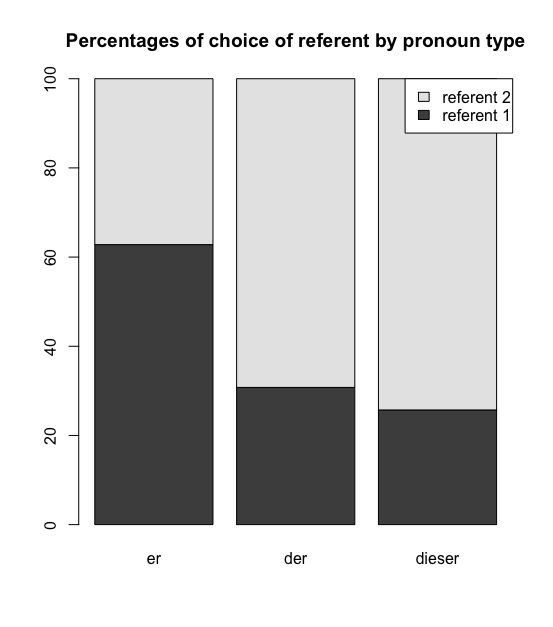
\includegraphics[width=\textwidth]{figures/a8FuchsSchumacher20200420-img001.jpg}
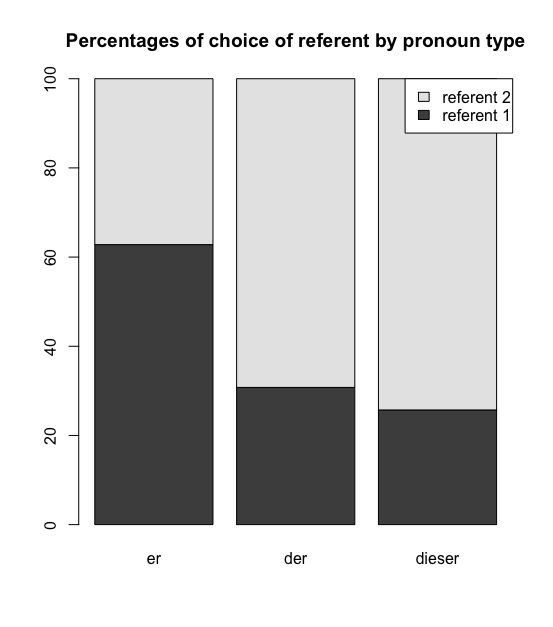
\includegraphics[height=.6\textheight]{figures/a8FuchsSchumacher20200420-img001.jpg} \caption{Percentage of reference resolution to first- and second-mentioned referent from first sentence for each pronoun type}
\label{fig:fuchs:1}
\end{figure}

\subsubsection{Referential shift potential – Remention capacity}\label{sec:fuchs:2.5.2}


\figref{fig:fuchs:2} shows how likely it is that any mention of an animate referent in the continuations refers back to the less prominent (i.e. second-mentioned) referent from the first context sentence. The figure shows the results depending on the pronoun type (\textit{er} vs. \textit{der} vs. \textit{dieser}). More specifically, the left panel shows the results obtained in those cases when the pronoun was interpreted towards the first-mentioned character from the first context sentence; the right panel shows the results obtained in those cases when the pronoun was interpreted towards the second-mentioned character in the first context sentence. When the pronouns were interpreted as referring to the less prominent character (right panel), all pronouns initiated a referential shift in subsequent discourse towards the previously less prominent character. These results hold even for the personal pronoun that has been claimed to maintain the current referential structure (e.g. \citealt{Abraham2002}). However, when the pronouns were interpreted as referring to the first-mentioned character, (numerical) differences between the different pronouns become apparent. When the demonstrative pronoun \textit{der} was interpreted as referring to the first-mentioned character, the second-mentioned character nevertheless appears to be accessible to a certain degree in the story continuations. By contrast, when the demonstrative pronoun \textit{dieser} was interpreted as referring to the first-mentioned character, the second-mentioned one appears to be less accessible in the story continuations. This (numerical) difference between \textit{der} and \textit{dieser} suggests that \textit{der} has a slightly bigger potential to change the prominence relations in discourse even when it is interpreted with respect to the more prominent referent. Similar to the analysis regarding the preferred referent of the pronouns, verb type did not significantly change the model results and is thus not represented in \figref{fig:fuchs:2}.

\begin{figure}
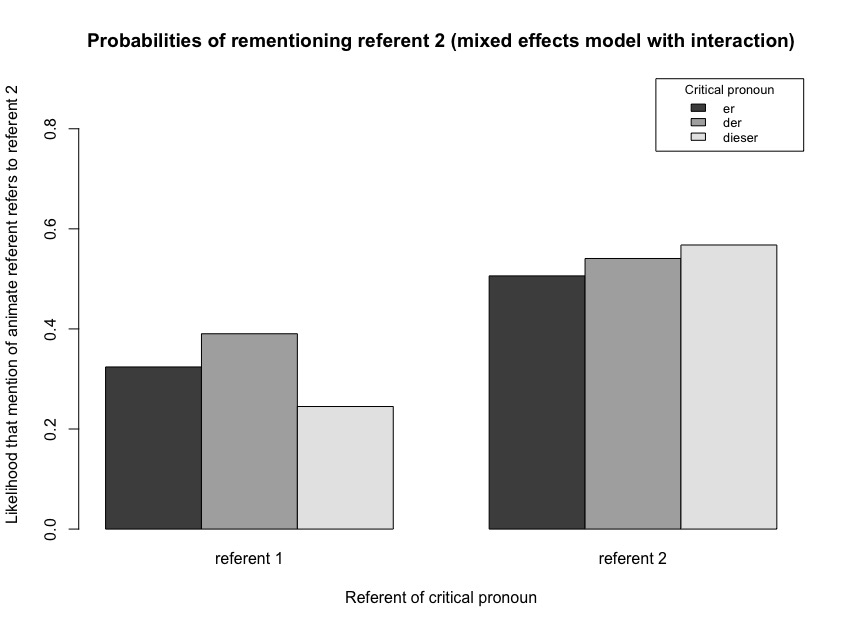
\includegraphics[width=\textwidth]{figures/a8FuchsSchumacher20200420-img002.jpg}
\caption{Probabilities (in percent) that any mention of an animate referent in story continuations refers to second-mentioned referent from the first sentence (depending on pronoun type and referent of pronoun)}
\label{fig:fuchs:2}
\end{figure}

The comparison between the model with a pronoun type by preferred referent interaction and the one containing the three-way interaction of preferred referent, pronoun type and verb type did not reveal a significant improvement of the model fit (likelihood-ratio test: \textit{p}~= 0.17).\footnote{R returned the warning message that the more complex model with the three-way interaction did not converge. The results of the model comparison should therefore be interpreted with caution. To double check, we ran the two models as Bayesian mixed models (using the R package brms \citep{Bürkner2017} with default priors) and compared them using Bayes factors. The results of this comparison also provide evidence for the reduced model without the three-way interaction (BF~= 0.002).} 

Statistical analyses of the predicted probabilities are thus reported for the model containing the interaction of pronoun type and preferred referent as fixed effects and random intercepts for items and participants. Participants were significantly more likely to choose to mention the second-mentioned character if they interpreted the critical pronoun as referring to the second-mentioned character from the first context sentence. This is indicated by a model with the same dependent variable (i.e. whether an animate referent in the continuations refers to \textit{Ref2} or not) and the variable referent of the critical pronoun (i.e. who they assumed the ambiguous pronoun referred to) as the only fixed effect (difference measured in logits: 0.93, SE~= 0.19, \textit{p} < 0.001). The differences within the two panels that are visible in \figref{fig:fuchs:2} did not reach statistical significance (possibly due to insufficient sample size). 

\subsubsection{Referential shift potential – Referential dynamics}\label{sec:fuchs:2.5.3}

As specified in \sectref{sec:fuchs:1.4.2}, we were also interested in whether the two demonstrative pronouns evoke different referential dynamics. \figref{fig:fuchs:3} illustrates how often the first- or second-mentioned referent is mentioned (in absolute numbers) at different points in the stories depending on the pronoun type. 

The top part of the figure illustrates how often the first-mentioned character is mentioned throughout the stories depending on the pronoun type. The x-axis refers to different points in the story. More specifically, it refers to the n\textsuperscript{th} mention of any animate referent in the story continuations. We enumerated all references to animate entities in the stories. The two animate characters from the first context sentence are the first two mentions and the pronoun in the second sentence is the third mention. The figure begins with the fourth mention of an animate entity and thus the first time the participants mentioned an animate referent. In the story continuation from \REF{ex:fuchs:5}, this would be the zero-pronoun marked on \textit{started}. For example, across all stories the fourth mention of an animate character refers in about five cases to the first-mentioned character when the target sentence contained \textit{dieser}. For all pronouns the number of references to the two characters declines towards the end. In this context it is important to note that the story continuations were of different length and therefore contained a different number of mentions of animate referents.   

Overall the top figure suggests that the personal pronoun \textit{er} (dashed line) evokes a higher number of references to the first-mentioned character over the course of the stories compared to the two demonstrative pronouns. This is especially clear from the beginning up until the 12\textsuperscript{th} mention of an animate referent. 

The lower part of the figure demonstrates how often the second-mentioned character from the context sentence is mentioned. Compared to the top part of the figure, it suggests that both types of demonstrative pronouns activate the second-mentioned character from the context sentence more often than the first-mentioned entity. Furthermore, the two demonstrative pronouns appear to boost reference to the second-mentioned character at different points in the stories. The number of mentions of the second-mentioned character in the context of \textit{dieser} (solid line) peaks at an earlier point in the development of the story and then declines. By contrast, in the context of \textit{der} (dotted line) the number of mentions of the second-mentioned character has an initial peak around the sixth mention and reaches its climax at a later point and, importantly, remains relatively high in the following period. 

\begin{figure}
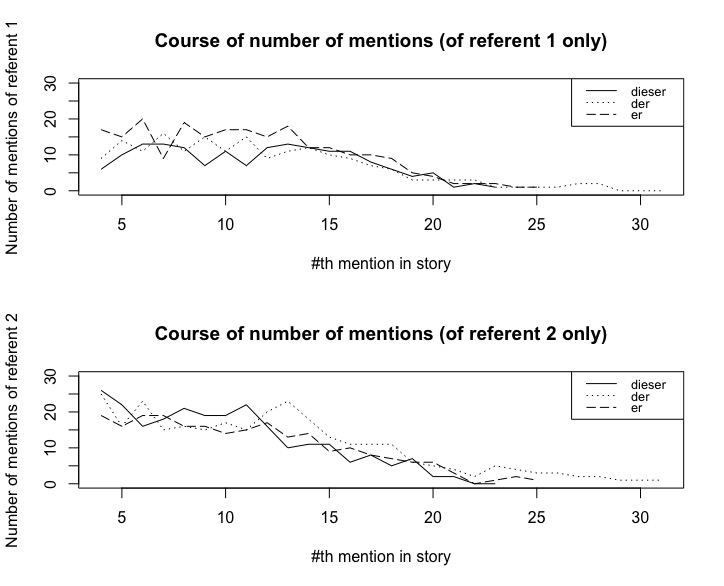
\includegraphics[width=\textwidth]{figures/a8FuchsSchumacher20200420-img003.jpg}
\caption{Number of times (absolute numbers) that the first- or second-mentioned character from the first sentence is mentioned at the n\textsuperscript{th} mention of any animate referent in story continuations}
\label{fig:fuchs:3}
\end{figure}

\section{General discussion}\label{sec:fuchs:3}

Our goal for this paper was two-fold. First, we wanted to compare the referential preferences of demonstrative pronouns to those of personal pronouns (choice of referent). Secondly, we wanted to investigate how far demonstrative pronouns initiate a referential shift in the following discourse (referential shift potential). 

\subsection{Choice of referent}\label{sec:fuchs:3.1}

The results for the interpretive preferences of the three types of pronouns investigated are fairly straightforward (see \figref{fig:fuchs:1}). The personal pronoun shows a preference for the first-mentioned proto-agent argument and both demonstrative pronouns reject this referent for the most part and have a robust preference for the second-mentioned proto-patient argument. These findings are in line with previous research on \textit{er} and \textit{der} (e.g. \citealt{BoschEtAl2003}; \citealt{SchumacherEtAl2016}). The results further provide new data on the interpretive preference of \textit{dieser.} Crucially, in context sentences with two referents and canonical (proto-agent before proto-patient) argument order, the two demonstrative pronouns pattern alike. Whether the resolution preferences for \textit{dieser} are triggered by an anti-agent preference (as, for example, shown by \citealt{SchumacherEtAl2016} for \textit{der}) or a last-mentioned preference \citep{ZifonunEtAl1997} cannot be determined on the basis of our experimental design. Note, however, that recent investigations question the last-mentioned preference that has been suggested for \textit{dieser} (\citealt{Lange2016}; \citealt{Özden2016}; \citealt{PatilEtAl2020}). In these experiments, contexts with non-canonical argument order were tested, as illustrated in \REF{ex:fuchs:6} (taken from \citealt{Özden2016}).

\ea\label{ex:fuchs:6}
\gll Den Direktor will der Schüler begrüßen. \\
     the.\textsc{acc} principle wants the.\textsc{nom} student to.welcome\\
\glt ‘The student wants to welcome the director.’
\z

In German non-canonical sentences, the less prominent thematic role (proto-patient) appears before the agent. According to the last-mentioned account, \textit{dieser} would simply select the last-mentioned entity which in this case is the agent. However, the participants in all three studies interpreted both demonstrative pronouns as referring to the first-mentioned patient. These results contradict a last-mentioned account and favour an account that is centred around thematic roles.

\subsection{Referential shift potential}\label{sec:fuchs:3.2}

With regard to our main research question of how pronouns influence the upcoming discourse, we were interested in two different aspects: we analysed how likely it is that any mention of an animate referent refers to the previously less prominent character and we looked at the referential dynamics of the unfolding stories. 

The results regarding how often the two discourse participants from the first context sentence were picked up in the continuations indicate differential effects. Which character is more likely to be mentioned in subsequent discourse appears to be influenced by the referent that was chosen for the pronoun (see \figref{fig:fuchs:2}). When the participants interpreted the pronoun as referring back to the less prominent character (see \figref{fig:fuchs:2}, right panel), this character appears to be more likely to be mentioned more frequently in the preceding discourse – irrespective of which pronoun the second context sentence contained. This suggests that when a less prominent character is chosen as referent for a subject pronoun and thus a referential shift is initiated, this has consequences for the development of subsequent discourse. This was expected for the two types of demonstrative pronouns, but not for the personal pronoun. However, personal pronouns have been shown to be generally more flexible in their referential choice (e.g. \citealt{BoschEtAl2007}; \citealt{SchumacherEtAl2016}). Therefore, it might not be surprising that they can initiate a referential shift in the few cases when they were initially understood as referring back to the less prominent character (remember that in around 35\% of the cases the personal pronoun from the second context sentence was understood as referring back to the less prominent patient, as illustrated in \figref{fig:fuchs:1}, and that only in these cases the personal pronoun initiated a referential shift in upcoming discourse). This suggests that the commitment to the less prominent referent was overall stronger.

However, when the participants interpreted the pronouns as referring back to the more prominent character, numerical differences between the different pronoun conditions became apparent (see \figref{fig:fuchs:2}, left panel). Interestingly, the demonstrative pronoun \textit{der} appears to have a small potential to shift the referential focus to the less prominent patient even when it was initially interpreted towards the more prominent agent. In contrast, the demonstrative pronoun \textit{dieser} does not show such an effect. We have to point out that these differences within the left panel of \figref{fig:fuchs:2} are statistically not significant, but display an interesting numerical trend. 

These findings provide initial support for an interdependence between interpretive preference and discourse change potential. The referential shift potential of different pronouns appears to be modulated by their interpretive preference in the first instance. It is thus not true across the board that demonstrative pronouns initiate a referential shift\footnote{See also \citet[73]{Weinert2011} who observed that demonstrative pronouns “are not rhematic per se”.} and that personal pronouns maintain the previously established prominence ranking. When the personal pronoun is interpreted as referring to the less prominent character, it can initiate a referential shift in favour of this less prominent character. Similarly, when the demonstrative pronoun \textit{dieser} is interpreted as referring to the more prominent character, it does not necessarily initiate a referential shift but might continue with the more prominent character in subsequent discourse. Based on our results, we therefore argue for a more differentiated view when it comes to describing the referential shift potential of different pronouns or other linguistic markers. 

Furthermore, the close investigation of referential dynamics (\figref{fig:fuchs:3}) across the story revealed interesting results. Different referential dynamics for the three pronouns could be observed. In the context of the demonstrative pronoun \textit{dieser}, the number of references to the less prominent character increased only for a short period of time. This mirrors the characterisation of \textit{dieser} as introducing a momentary interruption of a referential chain \citep{Weinrich1993}. In the context of \textit{der}, the number of references to the less prominent character remained relatively high throughout the story. This corroborates findings from spoken German where \textit{der} was used to establish a new centre of attention \citep{Ahrenholz2007}. 

\subsection{Strengths and limitations}\label{sec:fuchs:3.3}

While the referential shift potential can also be investigated through corpus research (see, for example, \citegen{Prince1981} corpus analysis of indefinite \textit{this}), the written or spoken version of the text continuation task allows for a more controlled approach to the study of different types of referential expressions. Given its experimental setup, the context sentences can be constructed in minimal pairs and other discourse-based factors can be kept stable. Moreover, since the use of certain referential forms in natural contexts may be too infrequent to draw conclusions about their functional contributions, a controlled experimental design allows the generation of sufficient data. In addition, in contrast to other more controlled approaches like reading time measures or eye tracking, this particular experimental task can be carried out without any additional equipment (in the written version) or with the aid of audio recording equipment (in the spoken version). It may thus serve as a valuable tool to test hypotheses linked to the discourse structuring potential of demonstratives and other discourse markers in settings where little technical equipment is available or for languages where large corpora are not available. 

Yet such a controlled setup is also subject to certain caveats. First, the contextual settings in the present experimental design introduced only two discourse referents (as has been the case in most experimental studies on pronoun resolution). Both demonstrative pronouns patterned alike and were interpreted as referring back to the less prominent proto-patient. However, future research should introduce contexts with more than two discourse referents in order to reveal potential differences between the two demonstrative pronouns that we could not capture with our reduced experimental setting (like reference to a less prominent referent vs. to the last-mentioned referent). A context with more than two discourse participants might also be informative with regard to our second research question of how the two demonstrative pronouns influence referential chains in subsequent discourse. As our context sentences make available only two referential candidates, the continuation task encourages participants to tell a story about these two individuals. As a result, likelihood of remention is high for both of these referents and participants often switch back and forth between the dominant characters in the story. Future research should therefore examine contexts with a larger set of potential candidates in order to see how the pronouns influence referential chains when more than two discourse participants are accessible. 

Another important issue is the question of whether the two types of demonstratives occur primarily in opposing registers and modalities and, following from this, how far our results can be applied to other contexts. In contrast to native speakers’ intuitions – that the demonstrative pronoun \textit{dieser} mainly occurs in written and/or formal contexts and \textit{der} is used in spoken and/or colloquial contexts – both types of demonstrative pronouns are reported to surface in spoken interactions between lecturers and students (\citealt{Ahrenholz2007}; \citealt{Weinert2007}). These results show that \textit{dieser} occurs in spoken contexts and that \textit{der} is not limited to informal contexts, as interactions between lectures and students might be considered rather formal. \citet{Weinrich1993} also argues that demonstratives from the \textit{der} paradigm should not be considered informal or colloquial. He points out that certain text types make the occurrence of certain types of referential expressions more likely (see also \citealt{Ahrenholz2007} for a similar account). By contrast, in a psycholinguistic experiment where participants had to insert a personal or demonstrative pronoun into a formal or informal text segment, \citet{PatilEtAl2020} found that participants preferred \textit{dieser} over \textit{der} in formal written contexts. Thus, there is so far not enough evidence regarding the role that different registers and modalities play in pronoun use. 

Hence the present findings may only be limited to the use of the two demonstratives in relatively formal written contexts. The two demonstratives may thus behave slightly differently in discrete contexts and modalities, but the available studies do not suggest that a preference for different registers and modalities alone can account for the differences between \textit{der} and \textit{dieser}. Therefore, follow-up studies are required. As a first step, a similar story continuation task in oral modality should be conducted where the participants hear the initial text segment and are then asked to continue the story orally. While experiments like the one presented in this chapter allow for a controlled approach to studying language comprehension and use, it would additionally be desirable to substantiate the findings on the basis of more natural, less controlled interactions between two or more discourse participants in written (e.g. chat rooms) and spoken contexts.  

\section{Conclusion}\label{sec:fuchs:4}

We have presented evidence from a story continuation task for different discourse functions of two types of German demonstrative pronouns compared with the personal pronoun. Regarding their interpretive preferences, the two types of demonstrative pronouns did not differ in their choice of referent and both selected the less prominent entity (i.e. the proto-patient). Our data further support previous findings that identified thematic role information to be a stronger cue during pronoun resolution than grammatical function (\citealt{StevensonEtAl1994}; \citealt{SchumacherEtAl2016}, \citeyear{SchumacherEtAl2017}), as in contexts with dative experiencer verbs the demonstrative pronouns referred back to the proto-patient/subject (and not the proto-agent/object). 

With respect to their referential shift potential, the two demonstrative pronouns revealed distinct patterns. The demonstrative pronoun \textit{der} showed a more robust referential shift potential. This became apparent from two observations: First, the demonstrative pronoun \textit{der} appears to be slightly more likely to initiate a shift towards the previously less prominent character even when it was initially understood as referring back to the more prominent character. Secondly, it showed a higher number of references to the less prominent character throughout the story. \textit{Dieser} by contrast appears to have a short-lived referential reorienting capacity. Further, we provided evidence that the referential shift potential is not an intrinsic property of demonstrative pronouns but is modulated by context-dependent factors such as to whom the demonstrative pronoun refers. Importantly, referential shift can also be displayed by the personal pronoun in those cases when it was initially interpreted as referring back to the less prominent character (though in these cases the participants might have processed it as a stressed personal pronoun). 

\subsection*{Acknowledgments}

This research has been funded by the German Research Foundation (DFG) as part of the SFB 1252 “Prominence in Language” (project number 281511265) in the project C07 “Forward and Backward Functions of Discourse Anaphora” at the University of Cologne. We would like to thank Julia Plechatsch, Hilde Gschossmann, Julia Veth and Celine Cuma for help with data collection and annotation. Furthermore, we would like to thank Eric Engel for setting up our annotation software and helpful suggestions concerning data analysis as well as Fahime Same for support with data extraction and Maximilian Hörl for support with data analysis. Furthermore, we would like to thank two anonymous reviewers and the editors of the volume for helpful comments and suggestions. 


\sloppy\printbibliography[heading=subbibliography,notkeyword=this]
\end{document}
